%!TEX root = paper.tex
%%%%%%%%%%%%%%%%%%%%%%%%%%%%%%%%%%%%%%%%%%%%%%%%%%%%%%%%%%%%%%%%%%%%%%%%%%%%%%%%
\section{Background}
\label{sec:background}


%%%%%%%%%%%%%%%%%%%%%%%%%%%%%%%%%%%%%%%%%%%%%%%%%%%%%%%%%%%%%%%%%%%%%%%%%%%%%%%%
\subsection{Service Costs of Gaming Platforms}

Price Models of:

\paragraph{Steam and PC in General}

\paragraph{Consoles}

\paragraph{Historical Example: OnLinve}


\paragraph{Geforce Now}
\url{http://shield.nvidia.com/game-streaming-with-geforce-now}
Kosten

\$7.99/mo + 200\$/€++ Hardware

Started in parts of Europe in Q4/2015

Spieleangebot

\$x Spiele im Paket

 + weitere/neuere zusätzlich mit Einmalbetrag

Leistung
Bandbreite? 

\paragraph{Playstation Now}
Streaming von PS3 Spielen auf PS4 und andere Sony-Geräte (als Rückwärtskompatibiliätslösung)
Kosten

(US/UK only?) Deuschlandbeta seit ~Q4/2015

\$ /mo + 330\$/€ (PS4) oder Sony TV + Controller
Extrakosten/Tagesleihgebühren für bestimmte ``bessere'' Spiele




%%%%%%%%%%%%%%%%%%%%%%%%%%%%%%%%%%%%%%%%%%%%%%%%%%%%%%%%%%%%%%%%%%%%%%%%%%%%%%%%
\subsection{Platform Provider Costs}
Backend/Service Requirements and Demands

%%%%%%%%%%%%
\subsubsection{CAPEX}

\begin{itemize}
	\item Regionale Data Center
	\item Gaming Server (GPU-Enabled)
	\item Entwicklungskosten für Software-Plattform(?)
\end{itemize}

\paragraph{Hardware}

\url{https://www.nvidia.com/object/cloud-gaming-gpu-boards.html}
\url{https://www.nvidia.com/object/grid-technology.html}


%%%%%%%%%%%%
\subsubsection{OPEX}

\paragraph{Verkehrsvolumen}

\begin{itemize}
	\item Internetanbindung?
	\item Caching of basic resources is probably not applicable?
\end{itemize}

\paragraph{Serverlaufzeiten}

\begin{itemize}
	\item Energie
	\item Verschleiß
	\item Wartungs- und Betriebspersonal oder Anmietung
	\item Frage: Rechnet sich Anmietung von Ressourcen bei großen generischen Rechenzentren? Annahme nein, da man selbst ein großer Anbieter wäre u. die Margin wegfallen. Auf der anderen Seite gibt es Hardware die für Games im Serverbereich besser skalieren? Wenn ja, kann umso mehr kein generischer Anbieter die Lösung sein
\end{itemize}

\paragraph{Spiele-Lizenzen und -Adaptionskosten (?)}
Modelannahme: Kosten pro Nutzung (realistisch eher in Blöcken verrechnet)





%%%%%%%%%%%%%%%%%%%%%%%%%%%%%%%%%%%%%%%%%%%%%%%%%%%%%%%%%%%%%%%%%%%%%%%%%%%%%%%%
\subsection{Data}

The leading question for the user side of the cost-benefit analysis is: ``How can we properly estimate the value a user gets from a specific service?'' with an additional question of ``What is the definition of value in this context?''

Simply counting the number of games one gets for a specific amount of money may be the easiest value metric but may also fall short. Therefore, this paper evaluates further approaches that also take game lengths and press review scores into account.

In order to achieve this, data had to be collected from various sources and merged into a consistent data base. All the scraping and merging code as well as the data itself can be found in the repositories at TODO to be verified by third parties. The following sections describe the individual data sources.

%%%%%%%%%%%%
\subsubsection{Steam API + SteamSpy Datensätze+Graphen}

Steam Sales:
Large seasonal sales (christmas, summer, lunar new year, halloween, fall, spring, ...) of many/most games on the platform usually rebates of 50\% and up.
Weekly sales
Daily sales
Weekend sales
Free weekends



\url{https://github.com/mas-ude/steam-data-stats} Steam + SteamSpy REST API Datensammler + ein paar Graphplotter (und eher ergebnislose Clustering-Versuche); für sinnvolle Analsyen müsste man dazu aber viel häufiger Datensätze generieren. Beispielausgaben:

CDF der Preise auf Steam (Juli ‘15) \ref{fig:steam-prices}

\begin{figure}[!t]
	\centering
	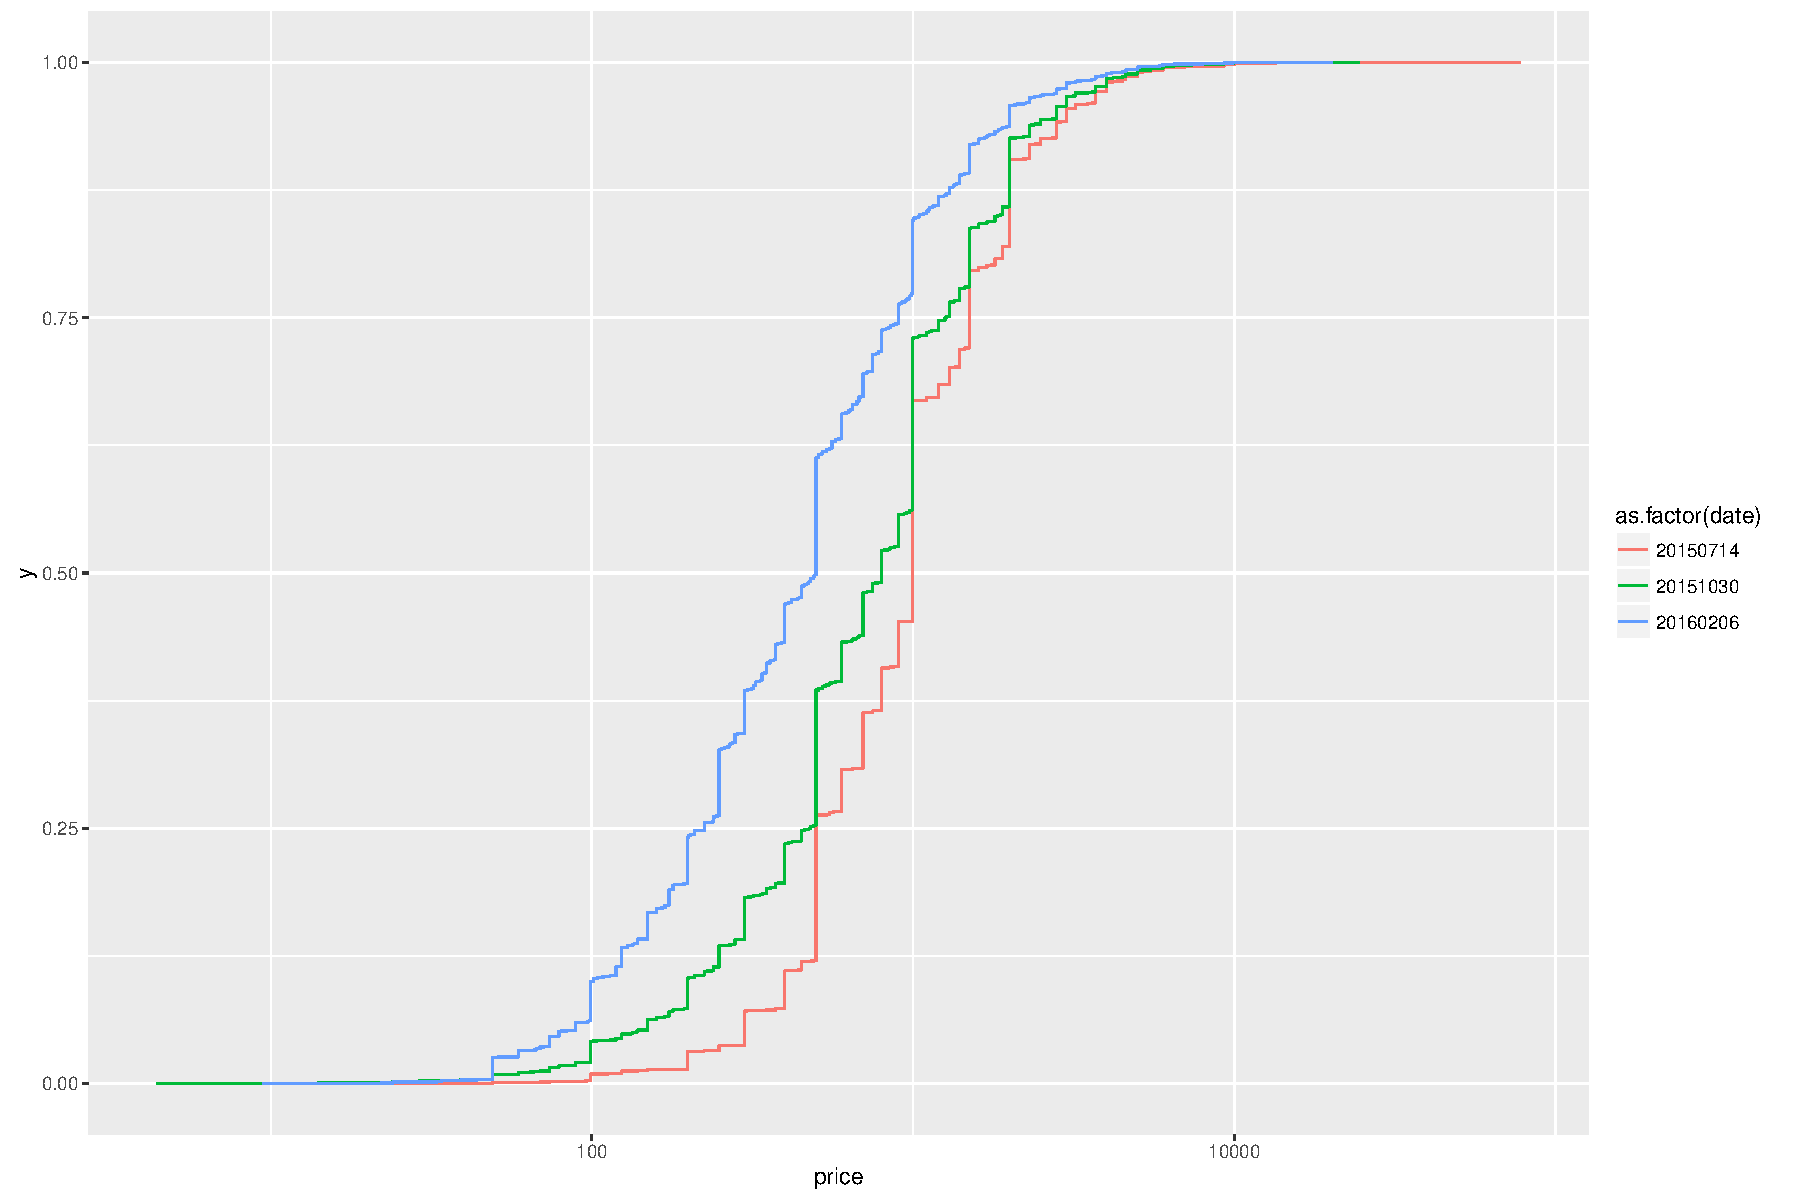
\includegraphics[width=1.0\columnwidth]{images/steam-prices.pdf}
	\caption{CDF of games on the steam platform at two distinct dates.}
\label{fig:steam-prices}
\end{figure}

Violinenplot der durchschnittlichen Spielzeit aufgeteilt auf unterschiedliche Preiskategorien. \ref{fig:steam-cost-vs-playtime-violin}

\begin{figure}[!t]
	\centering
	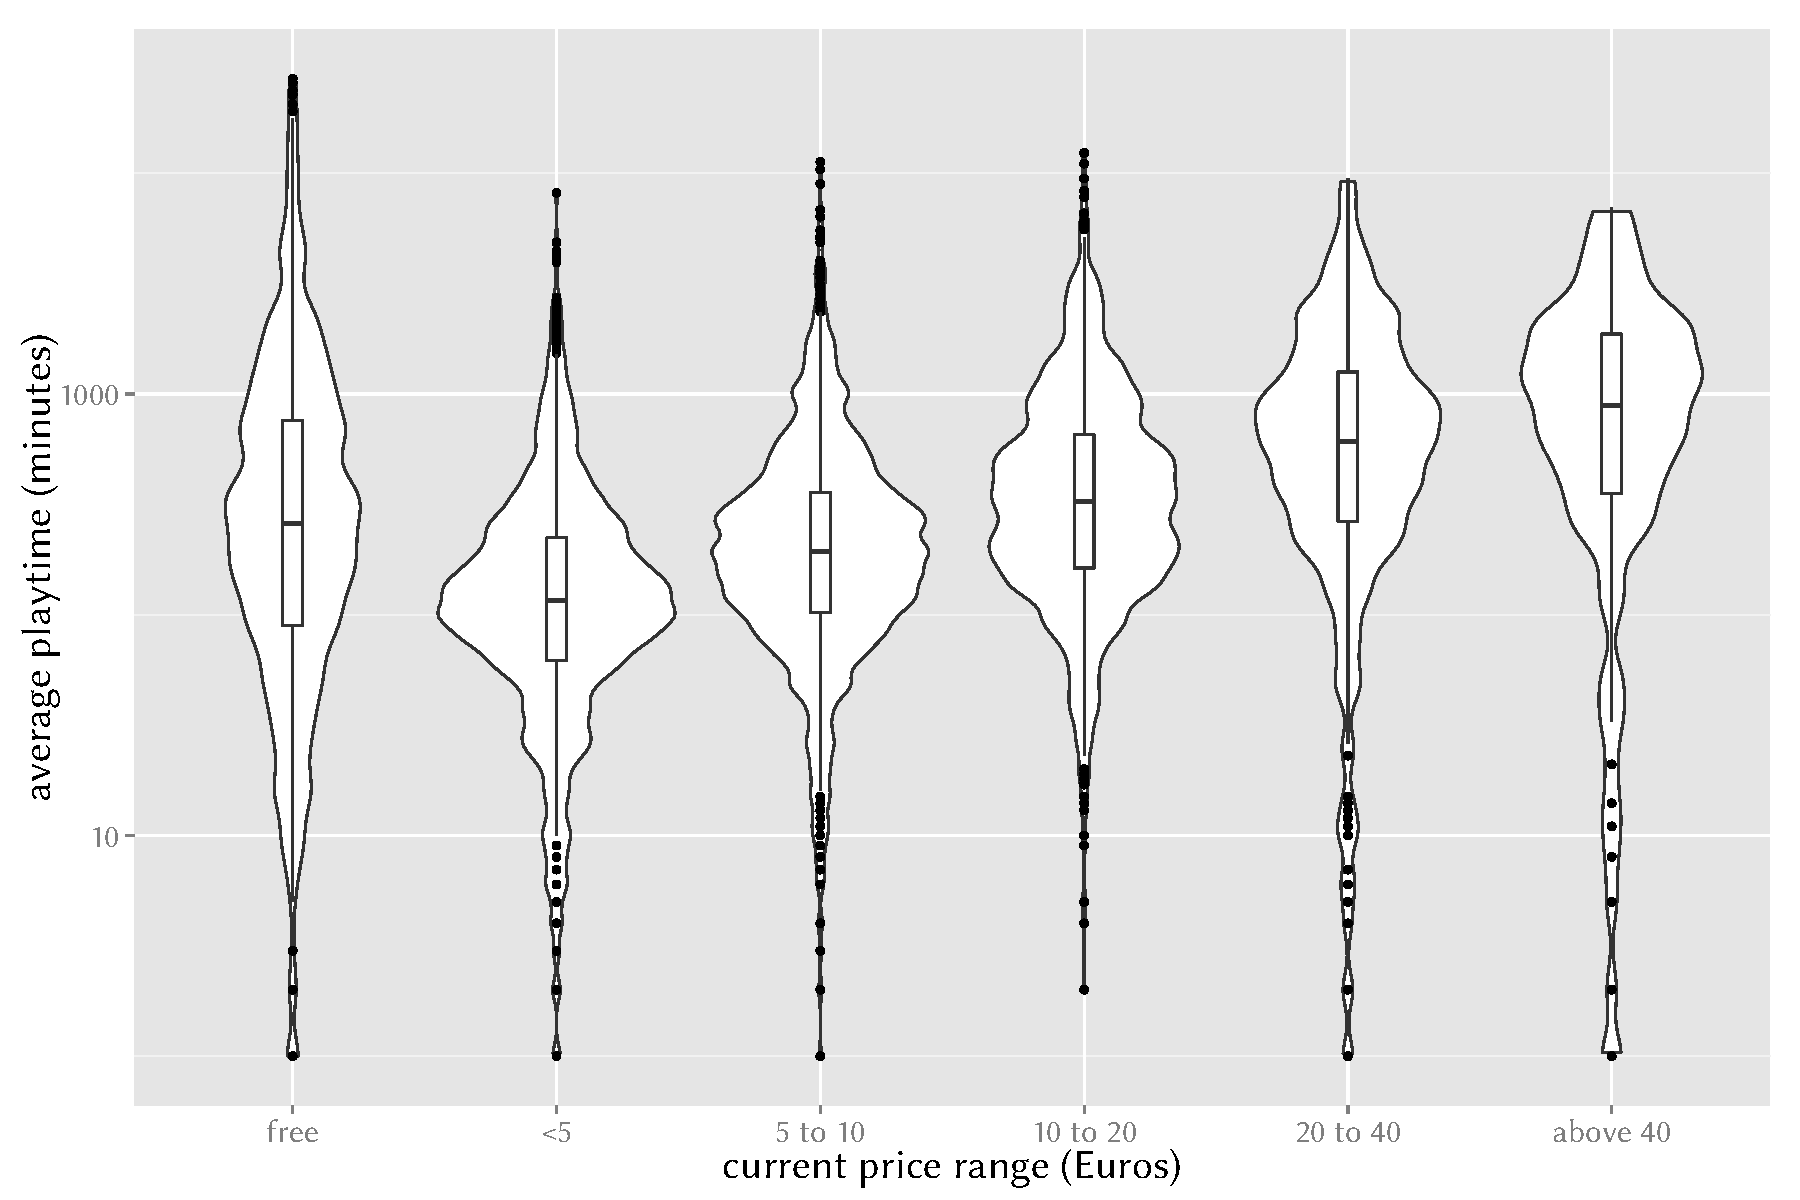
\includegraphics[width=1.0\columnwidth]{images/steam-cost-vs-playtime.pdf}
	\caption{Violin plot of the average playtime (as recorded by SteamSpy) of games categorized by their prices.}
\label{fig:steam-cost-vs-playtime-violin}
\end{figure}

%%%%%%%%%%%%
\subsubsection{HowLongToBeat Data}

Data scraped from \url{howlongtobeat.com}. This site allows for manual reporting of playthrough times of games on any platform. Times are separated into different play styles (e.g. ``main story'', ``completionist'') and only an aggregated time is shown. For this analysis only the average playtime of all play styles is taken into account.
It should however be stressed again, that this is a self-reporting site without strong validity checks. This has to be considered when contemplating the accuracy and validity of the data.

\begin{figure}[!t]
	\centering
	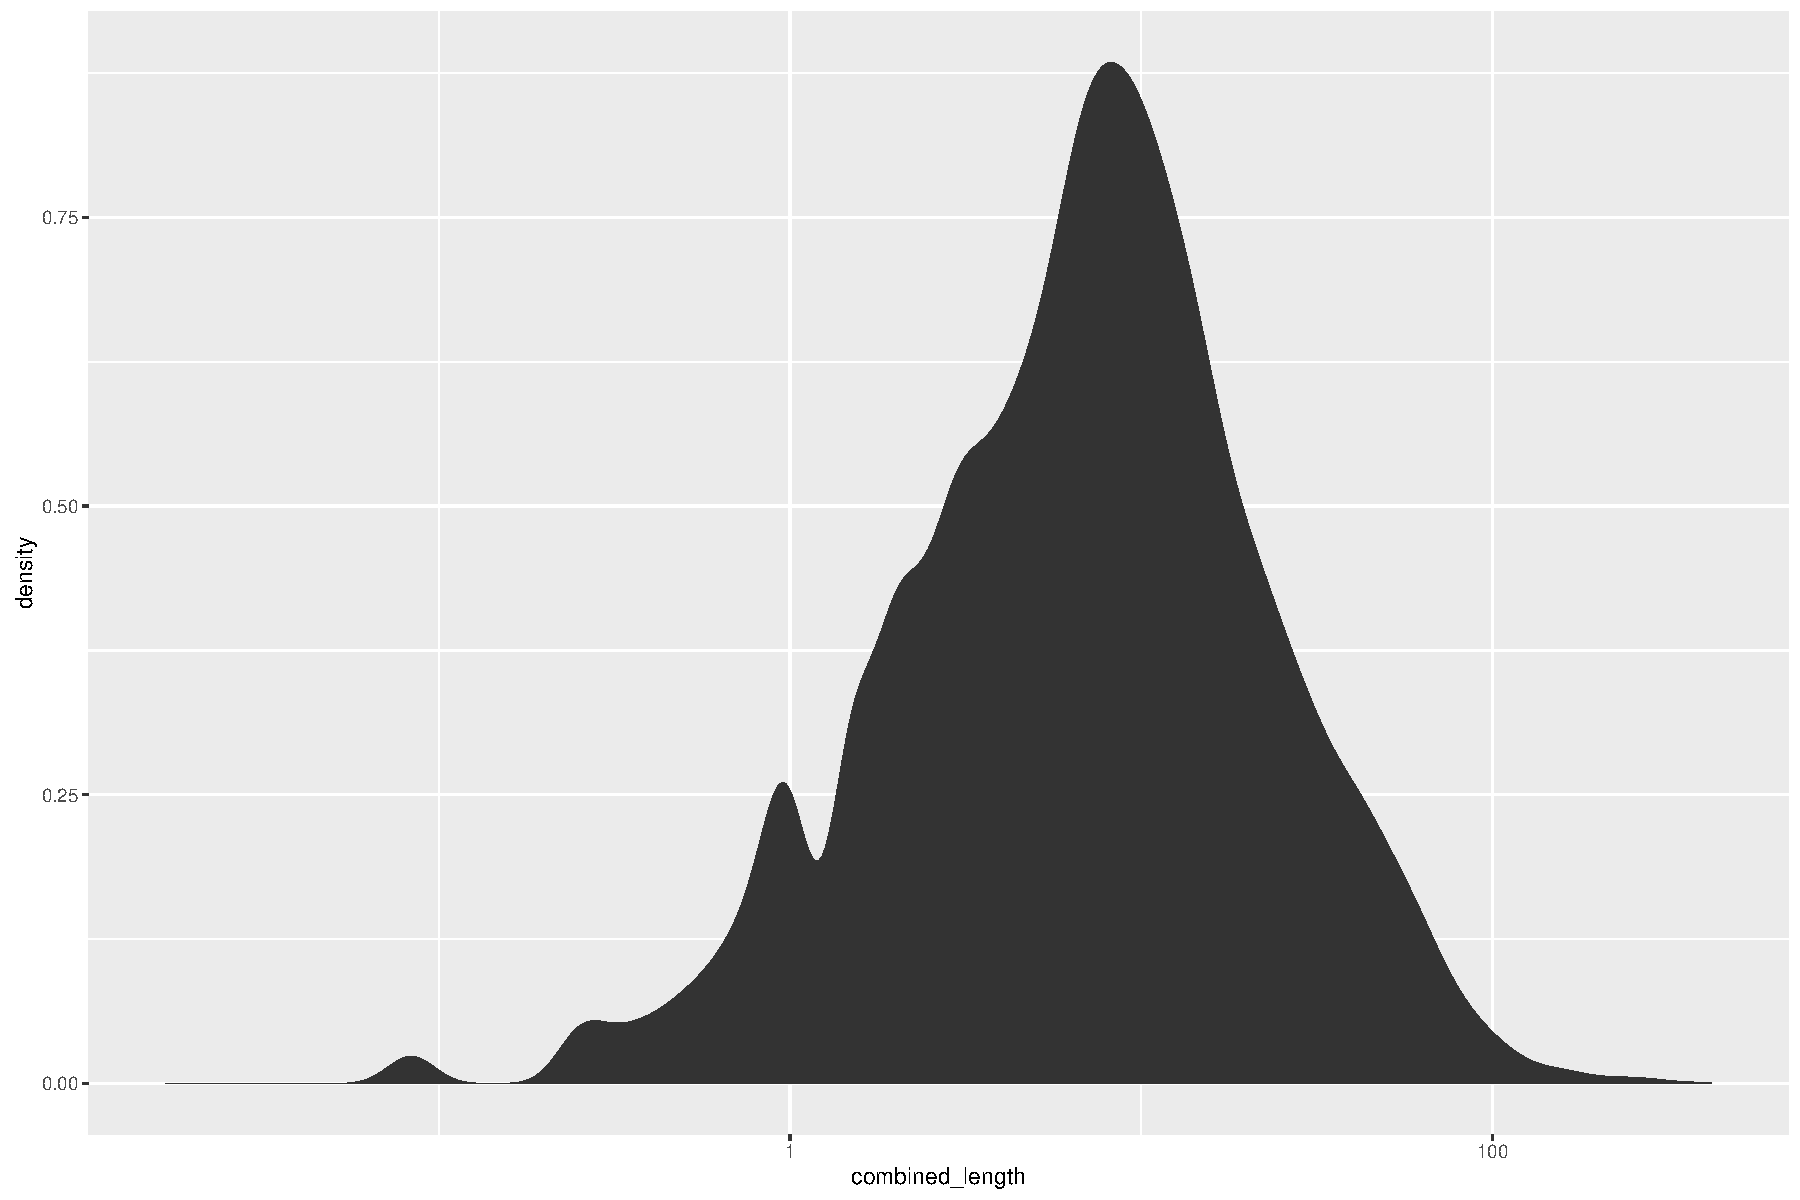
\includegraphics[width=1.0\columnwidth]{images/gamelengths-density.pdf}
	\caption{Density plot of the average game lengths over all play styles.}
\label{fig:gamelengths-density}
\end{figure}

Nonetheless, the distribution of game lengths from this set can still be worth to look at in the context of putting value to games for consumers of different platforms. As seen in Figure~\ref{fig:gamelengths-density} the play lengths vary greatly, with the median at \SI{7.5}{\hour} and a long tail of long play times reaching \SI{420}{\hour}.


%%%%%%%%%%%%
\subsubsection{Metacritic Data}

Game lengths can not only serve as an indicator of the amount of content a game has to offer, but can also serve as an engagement metric to estimate a user's amount of satisfaction. More fitting engagement metrics could also be employed.

% TODO: include or compare with data from opencritic.com as soon as their API is public/usable

\begin{figure}[!t]
	\centering
	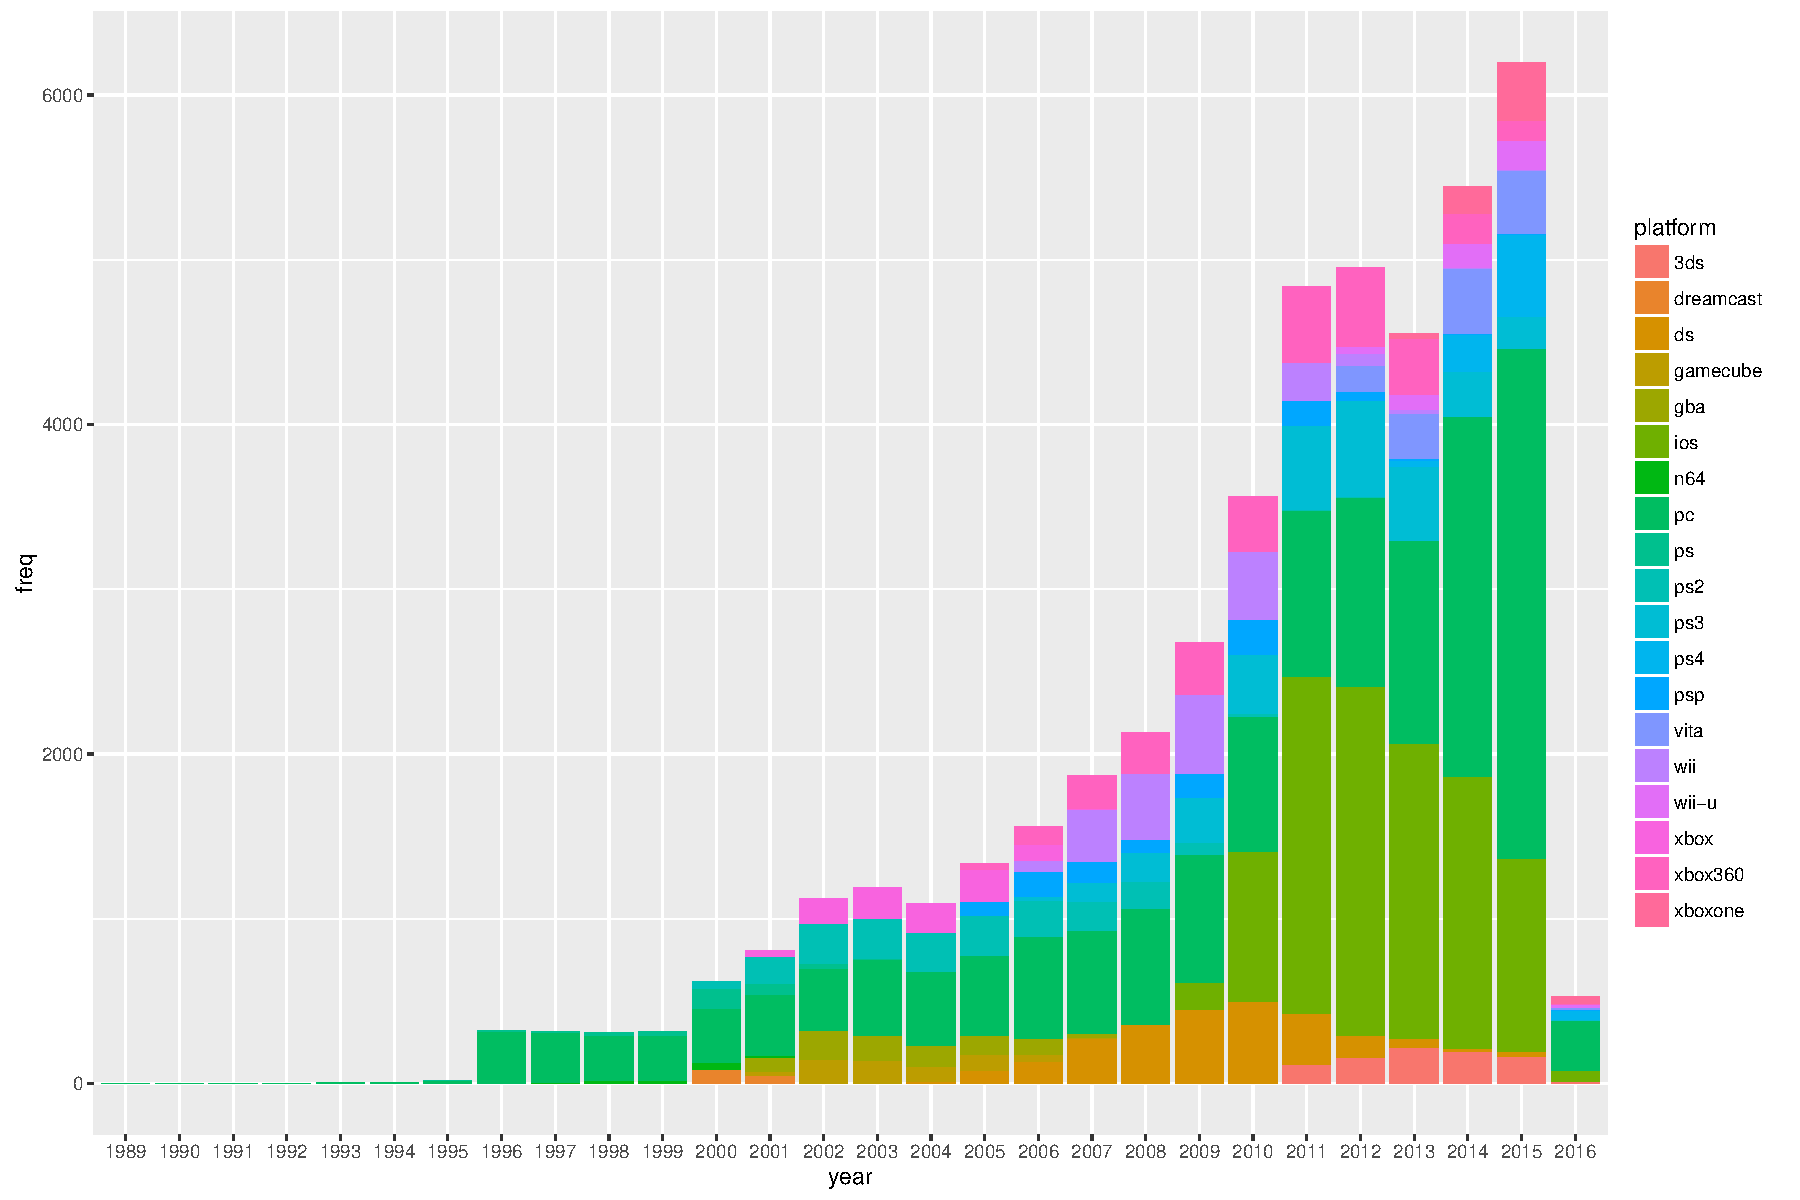
\includegraphics[width=1.0\columnwidth]{images/releases-per-year.pdf}
	\caption{Number of game releases per platform according to the Metacritic data.}
\label{fig:releases-per-year}
\end{figure}




